\chapter{Utilizzo del prodotto}\label{chap:istruzioni}
\section{Documenti}\label{sec:documenti}
\subsection{Aggiunta documento}
Per aggiungere un documento, cliccare sul pulsante "Aggiungi documento" presente nel menù a sinsitra.
\begin{figure}[h!]
    \centering
    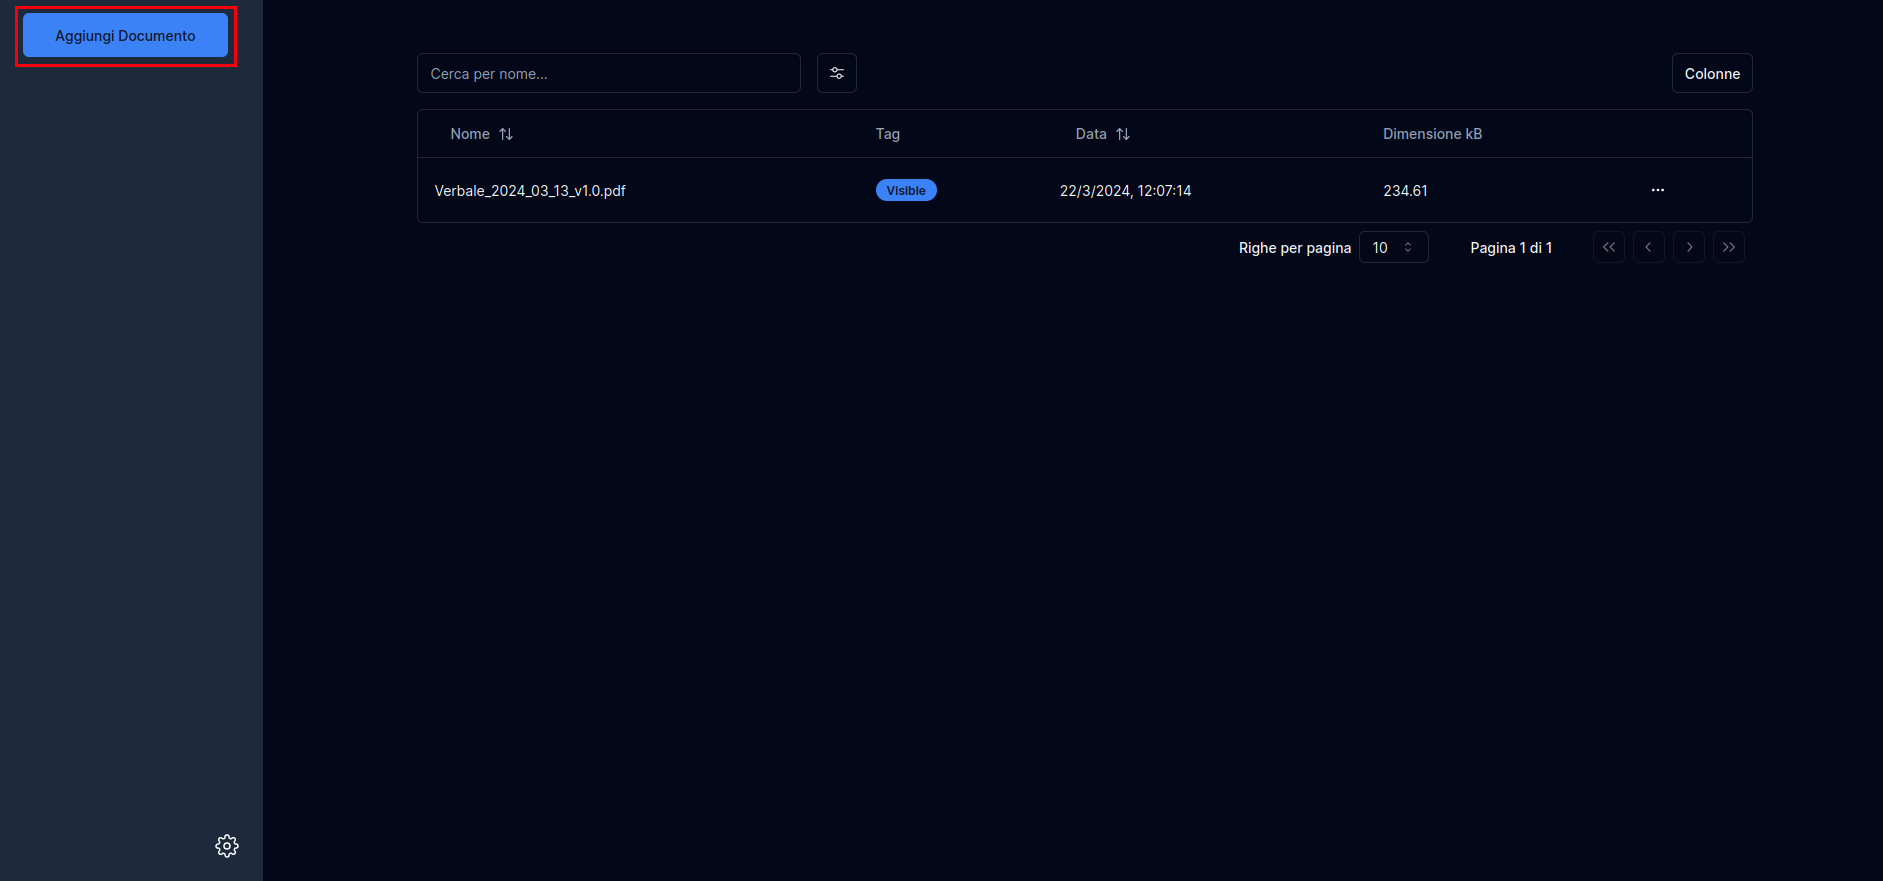
\includegraphics[width=0.8\textwidth]{schermatadocaggiungi.png}
    \caption{Aggiungi documento nel menù}\label{fig:adddocs}
\end{figure}
\\Si aprirà una finestra da cui si potrà selezionare il file da caricare trascinandolo o scegliendolo dai file in sistema.
\begin{figure}[h!]
    \centering
    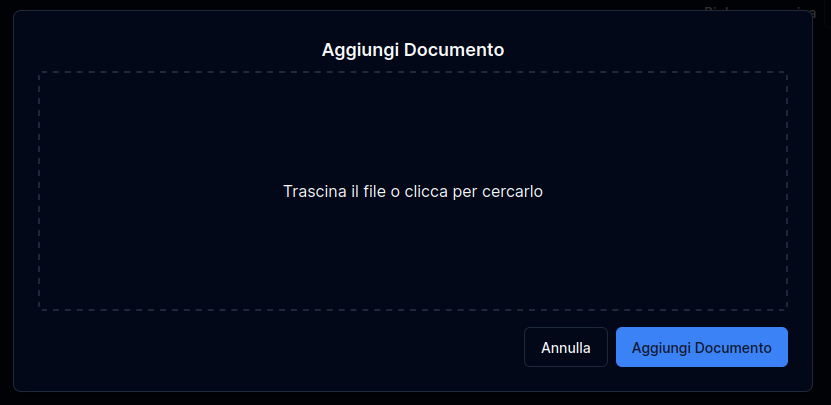
\includegraphics[width=0.6\textwidth]{dialogadd.png}
    \caption{Dialog aggiunta documento}\label{fig:dialogadd}
\end{figure}
\\Infine, cliccando su "Aggiungi documento", il documento verrà aggiunto alla lista dei documenti consultabili con il modello selezionato.
\begin{figure}[h!]
    \centering
    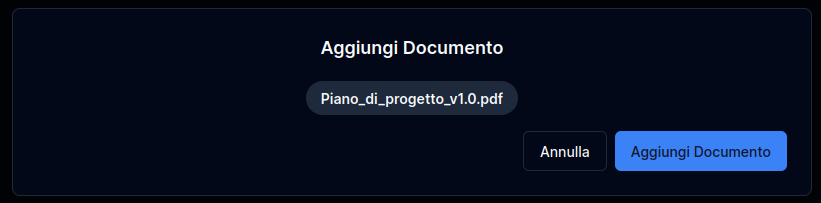
\includegraphics[width=0.6\textwidth]{docadd.png}
    \caption{Conferma aggiunta documento}\label{fig:confirmadd}
\end{figure}
\\Importante ricordare che i documenti caricati usando un modello locale non possono essere interrogati con il chatbot che utilizza OpenAI e viceversa.
\subsection{Ricerca documenti}
Nella parte superiore della sezione documenti è presente una barra di ricerca, in cui è possibile cercare documenti per nome o per data.
\begin{figure}[h!]
    \centering
    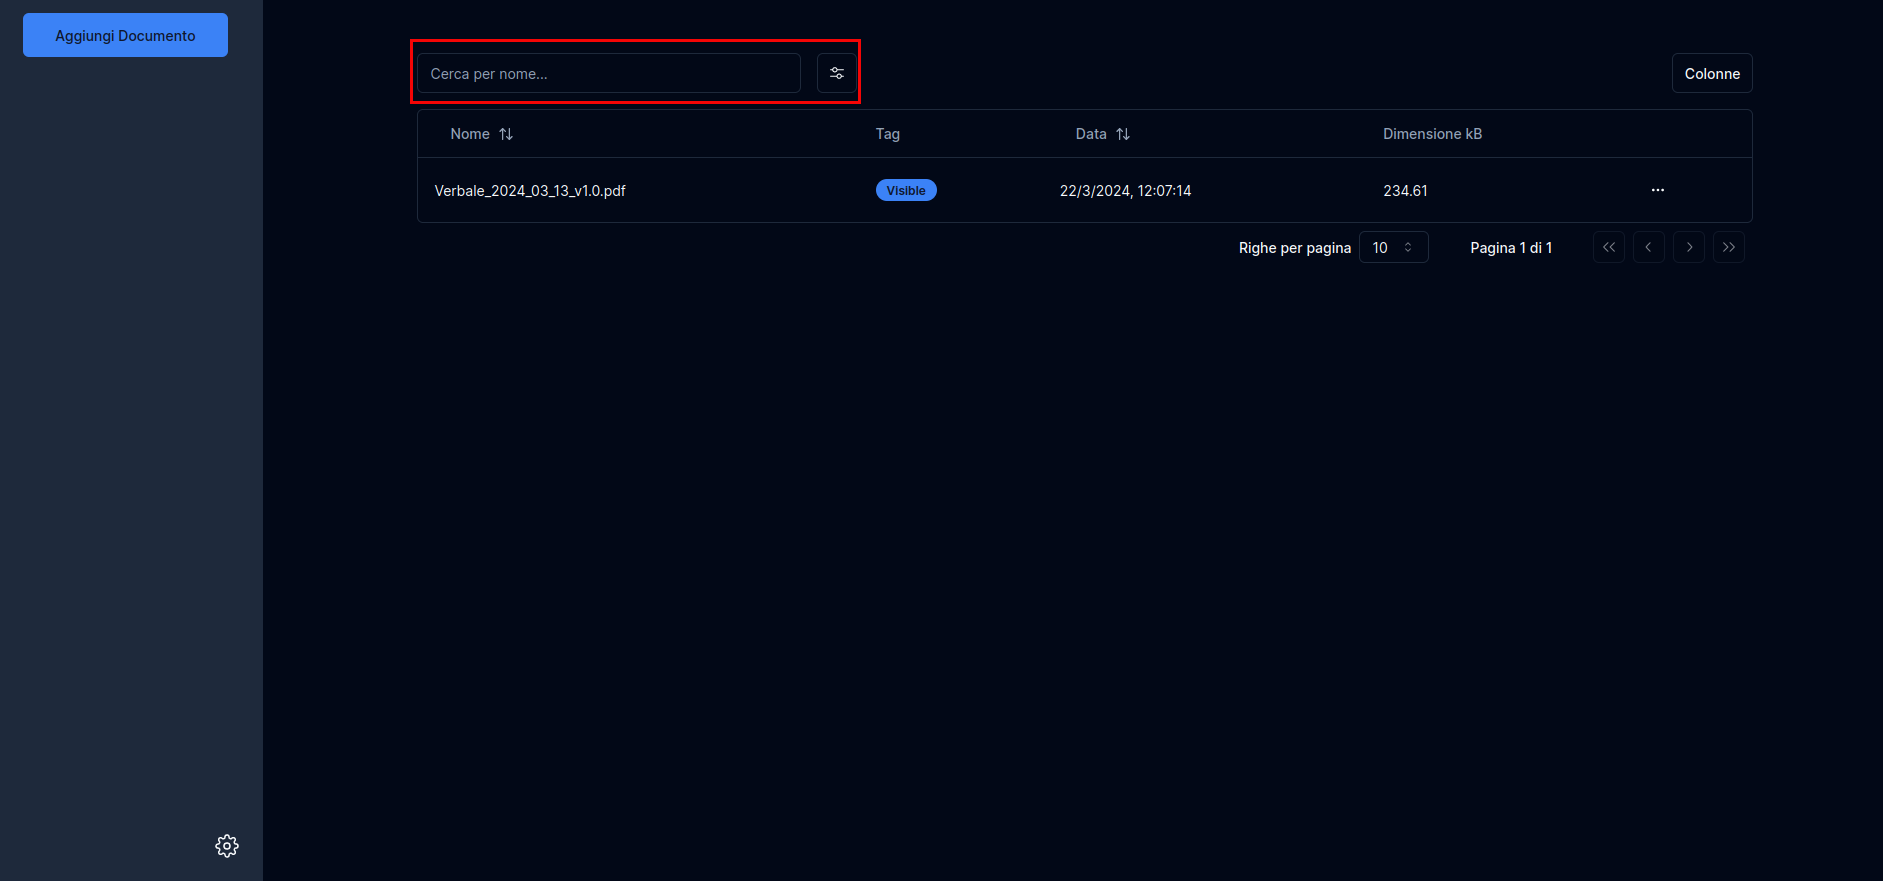
\includegraphics[width=0.75\textwidth]{schermatadocsearch.png}
    \caption{Barra ricerca documenti}\label{fig:searchdocs}
\end{figure}
\\Cliccando sul pulsante accanto alla barra di ricerca, è possibile scegliere il criterio con cui effettuare la ricerca.
\begin{figure}[h!]
    \centering
    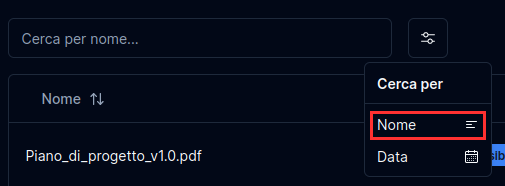
\includegraphics[width=0.56\textwidth]{cercadocnome.png}
    \caption{Cerca documento per nome}\label{fig:searchdocsname}
\end{figure}
\begin{figure}[h!]
    \centering
    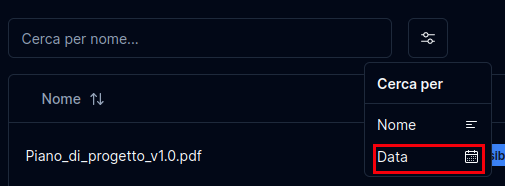
\includegraphics[width=0.56\textwidth]{cercadocdata.png}
    \caption{Cerca documento per data}\label{fig:searchdocsdate}
\end{figure}
\subsection{Impostazioni documento}
Cliccando sul pulsante a tre puntini accanto al documento, si aprirà un menù da cui è possibile scegliere tre diverse opzioni.
\begin{figure}[h!]
    \centering
    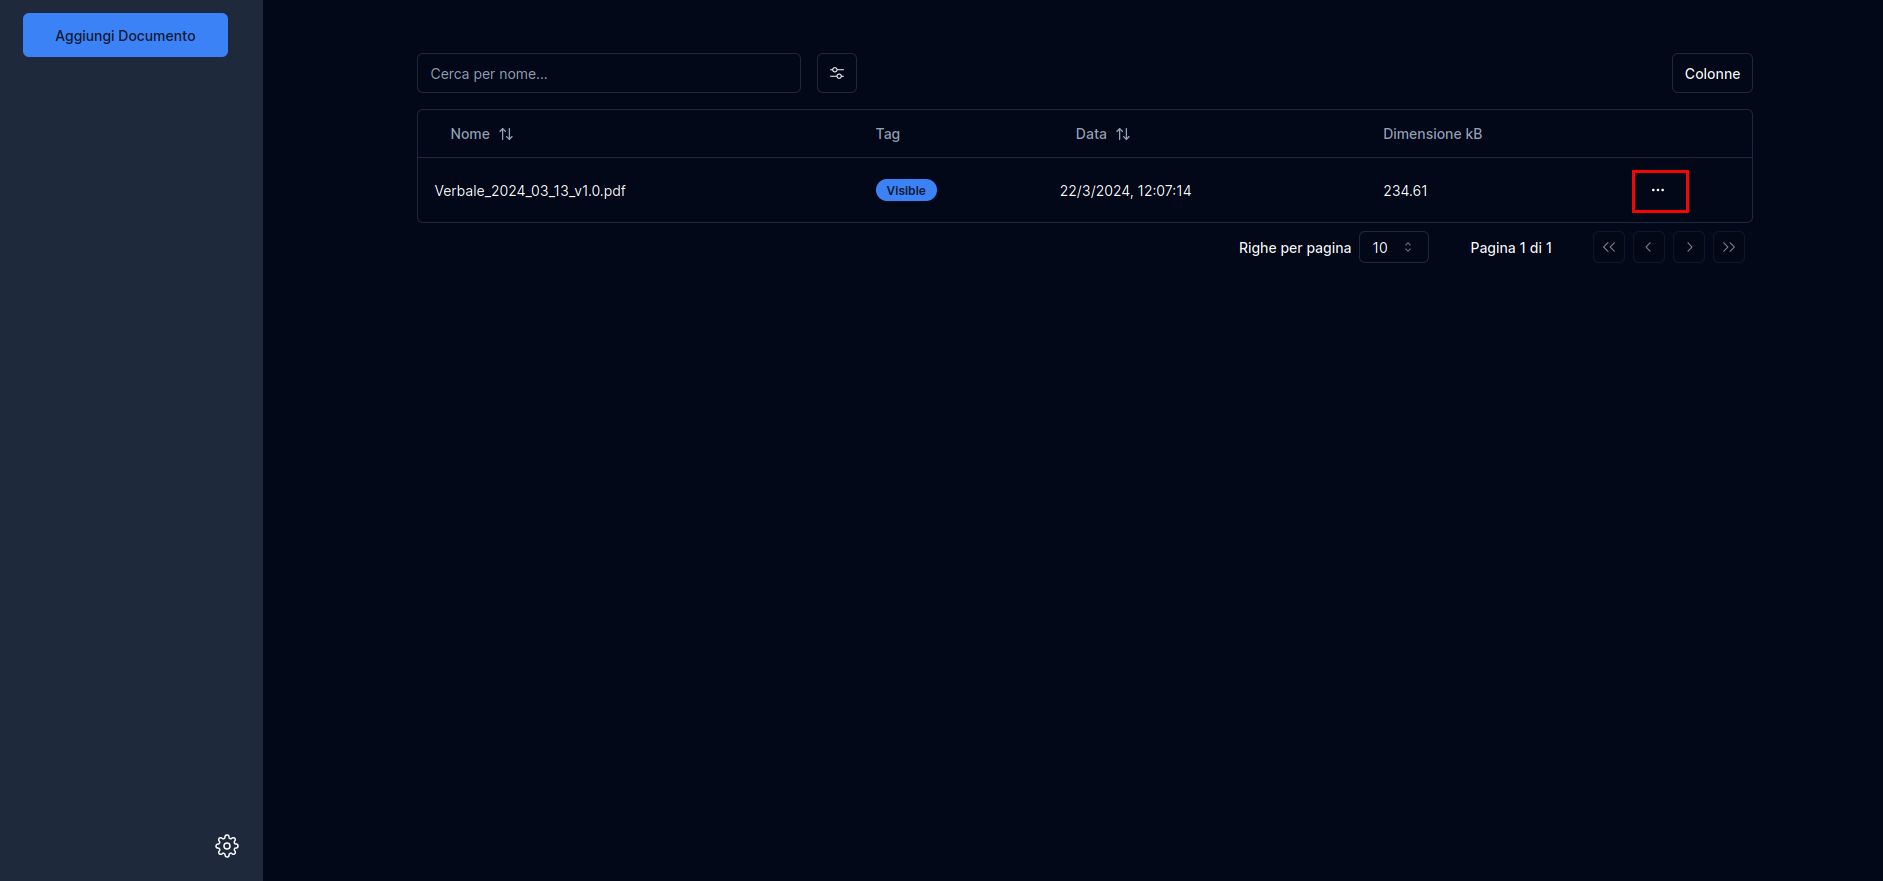
\includegraphics[width=0.72\textwidth]{schermatadoctrepunti.png}
    \caption{Menù documento}\label{fig:menudocs}
\end{figure}
\subsubsection{Visualizzazione documento}
Cliccando su "Visualizza" sarà possibile visualizzare il documento caricato. In caso si tratti di un pdf verrà aperto in un'altra scheda, altrimenti, se il file caricato è di un qualsiasi altro formato supportato dall'applicazione, verrà scaricato.  
\begin{figure}[h!]
    \centering
    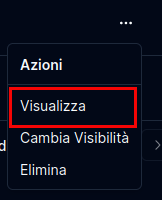
\includegraphics[width=0.16\textwidth]{menuactiondocvisualizza.png}
    \caption{Visualizza documento}\label{fig:seedocs}
\end{figure}
\subsubsection{Modifica visibilità documento}
Cliccando su "Cambia visibilità" il documento verrà reso visibile o meno. Importante ricordare che è possibile effettuare domande solo su documenti visibili e che un documento non visibile non è eliminato dal database, ma solo nascosto.
\begin{figure}[h!]
    \centering
    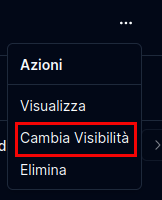
\includegraphics[width=0.16\textwidth]{menuactiondocvisibility.png}
    \caption{Modifica visibilità documento}\label{fig:visibilitydocs}
\end{figure}
\subsubsection{Eliminazione documento}
Cliccando su "Elimina" il documento verrà eliminato dal database e non sarà più possibile fare domande sul contenuto di quel documento.
\begin{figure}[h!]
    \centering
    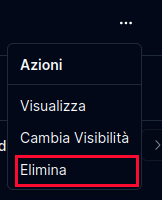
\includegraphics[width=0.16\textwidth]{menuactiondocdelete.png}
    \caption{Elimina documento}\label{fig:deletedocs}
\end{figure}
\\Per evitare eliminazioni accidentali, verrà richiesta una conferma prima di procedere.
\begin{figure}[h!]
    \centering
    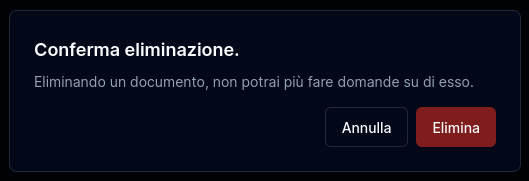
\includegraphics[width=0.6\textwidth]{confirmdeletedoc.png}
    \caption{Conferma eliminazione documento}\label{fig:dialogdelete}
\end{figure}   
\subsection{Impostazioni tabella}
\subsubsection{Colonne}
Cliccando sul pulsante "Colonne" sopra la tabella si aprirà un menù a tendina. 
\begin{figure}[h!]
    \centering
    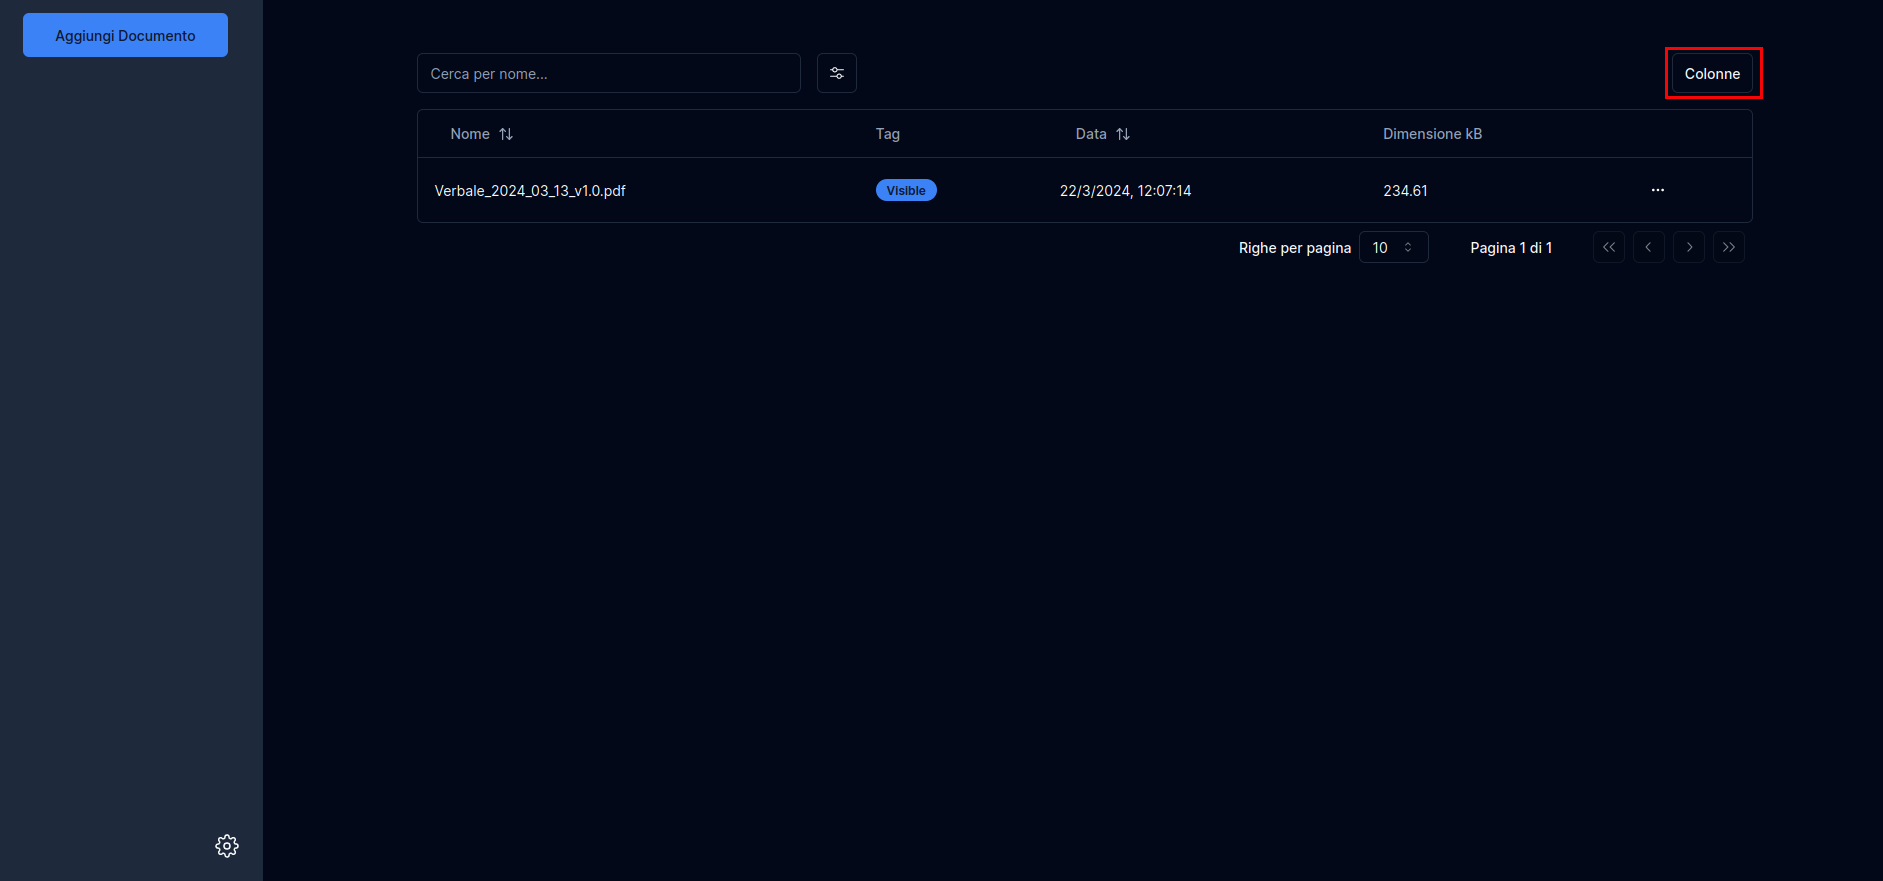
\includegraphics[width=0.8\textwidth]{schermatadocoloumns.png}
    \caption{Impostazioni tabella}\label{fig:settingtable}
\end{figure}
\\Da lì è possibile scegliere quali colonne visualizzare nella tabella dei documenti.
\begin{figure}[h!]
    \centering
    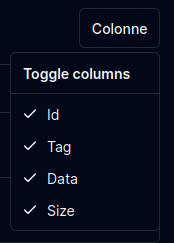
\includegraphics[width=0.25\textwidth]{visualizzacoldoc.png}
    \caption{Colonne tabella}\label{fig:coltable}
\end{figure}
\subsubsection{Righe}
È possibile scegliere di ordinare le righe della tabella in base a nome o data cliccando sulle frecce a lato dei titoletti. Inoltre, è possibile scegliere quante righe visualizzare e, grazie alle frecce in basso a destra, è possible navigare tra le eventuali pagine.
\begin{figure}[h!]
    \centering
    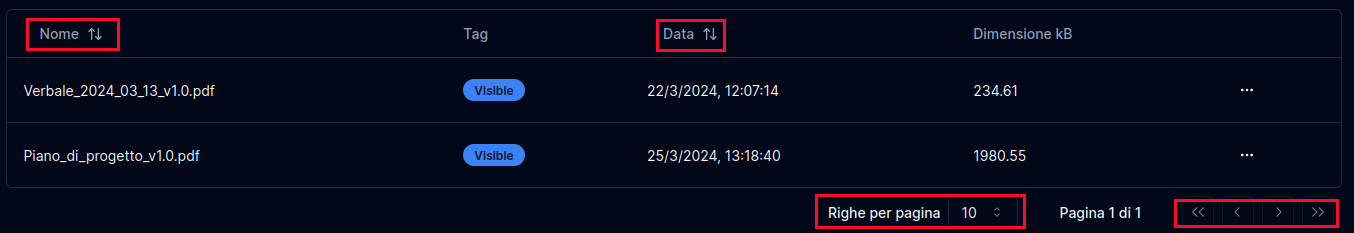
\includegraphics[width=0.8\textwidth]{visualizzaorderdoc.png}
    \caption{Righe tabella}\label{fig:rowtable}
\end{figure}
\subsection{Impostazioni applicazione}
Cliccando sulla rotellina presente nel menù di sinistra si apriranno le impostazioni dell'applicazione.
\begin{figure}[h!]
    \centering
    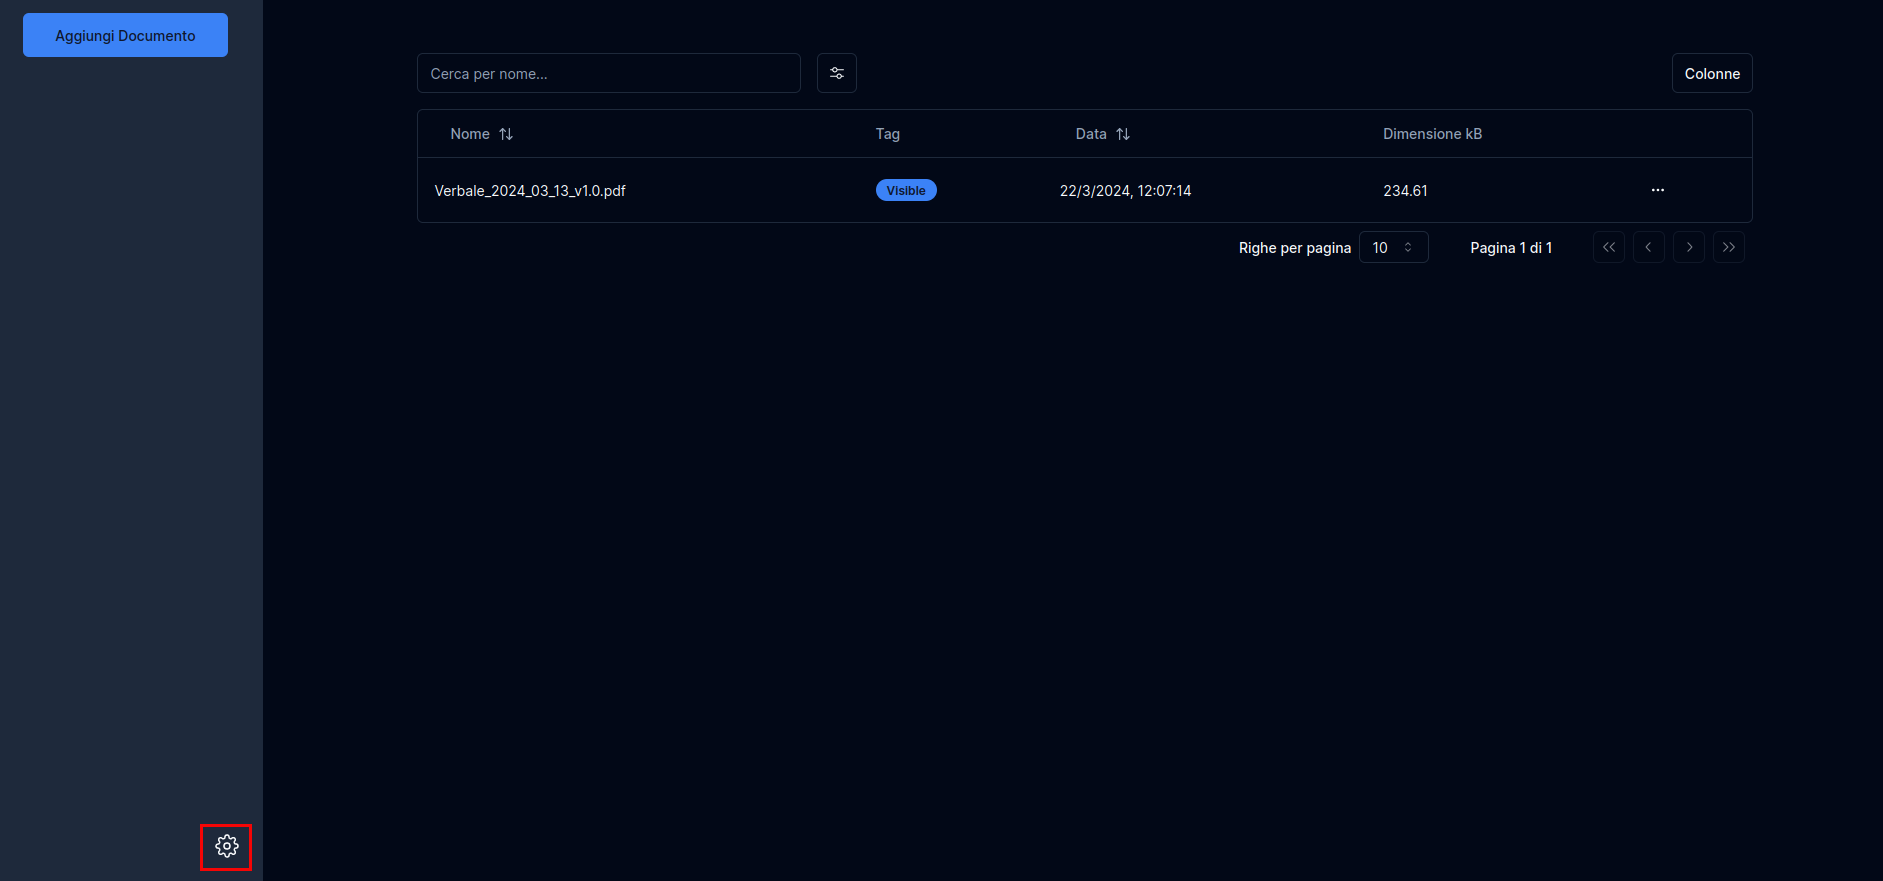
\includegraphics[width=0.8\textwidth]{schermatadocsetting.png}
    \caption{Impostazioni dell'applicazione}\label{fig:settingdoc}
\end{figure}
\subsubsection{Modifica modello}
Dalle impostazioni è possibile scegliere il modello con cui fare domande sui documenti. Importante ricordare che i documenti caricati usando un modello locale non possono
essere interrogati con il chatbot che utilizza OpenAI e viceversa.
\begin{figure}[h!]
    \centering
    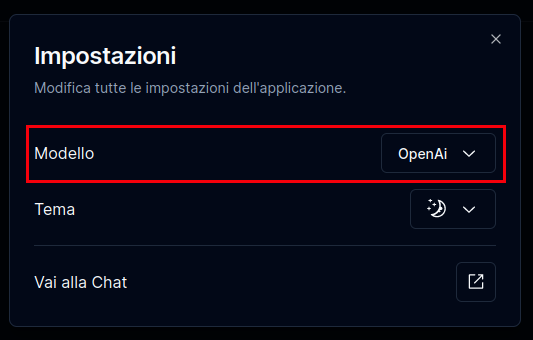
\includegraphics[width=0.364\textwidth]{settingdocmodel.png}
    \caption{Cambio modello}\label{fig:settingdocmodel}
\end{figure}
\subsubsection{Modifica tema}
È possibile cambiare il tema dell'applicazione selezionando tra modalità dark (rappresentata dalla luna) e modalità light (indicata dall'icona del sole).
\begin{figure}[h!]
    \centering
    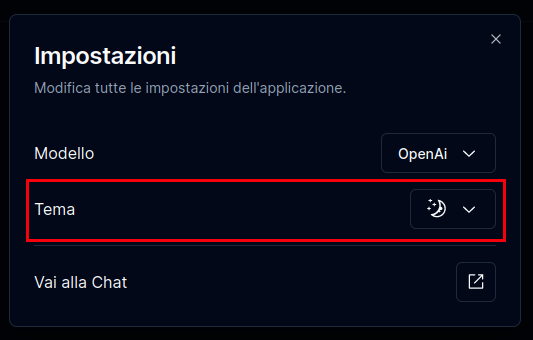
\includegraphics[width=0.364\textwidth]{settingdoctheme.png}
    \caption{Cambio tema}\label{fig:settingdoctheme}
\end{figure}
\subsubsection{Cambio pagina}
Per passare alla pagina chat basta cliccare sul pulsante "Vai alla chat" presente in fondo alle impostazioni.
\begin{figure}[h!]
    \centering
    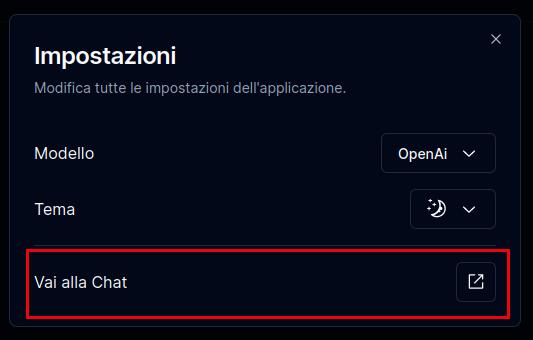
\includegraphics[width=0.364\textwidth]{settingdocchange.png}
    \caption{Vai alla pagina chat}\label{fig:changepage}
\end{figure}

\newpage
\section{Chatbot}\label{secchatbot}

\subsection{Interazione chatbot}
\subsubsection{Inserimento domanda}
Per interagire e interrogare il chatbot è possibile inserire il testo della domanda nella barra posta nella parte bassa dell'applicazione.
\begin{figure}[h!]
    \centering
    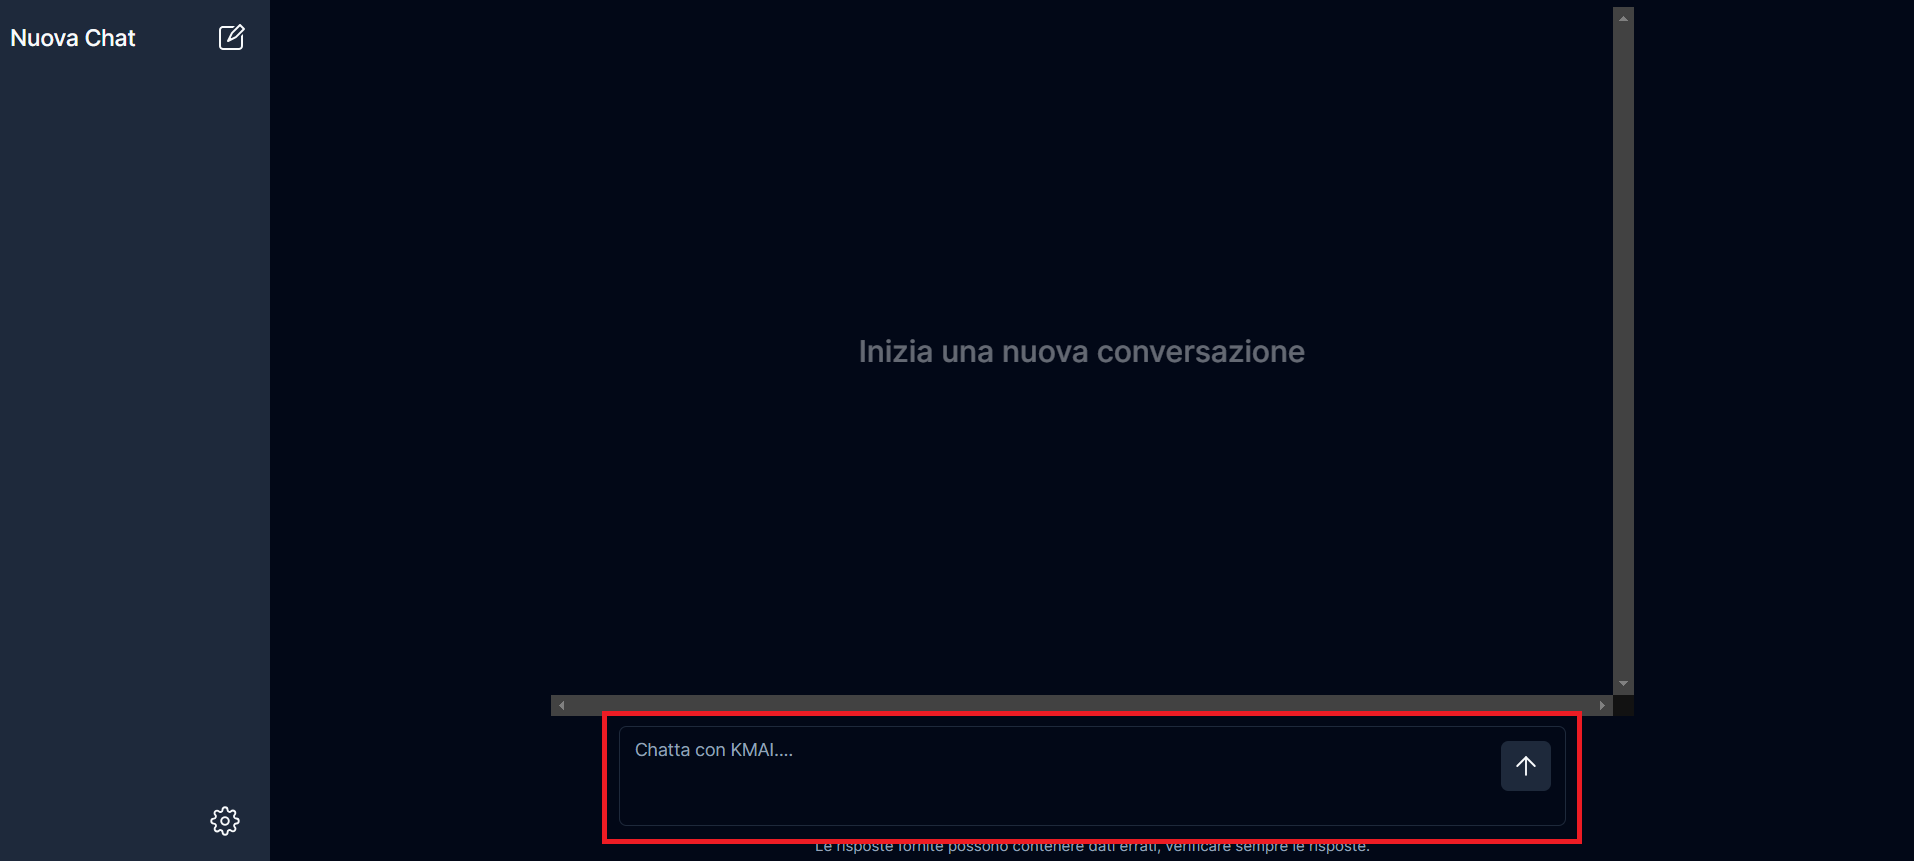
\includegraphics[width=0.8\textwidth]{inserttextchat.png}
    \caption{Inserimento domanda}\label{fig:inserttextchat}
\end{figure}
\subsubsection{Invio domanda}
Una volta inserito il testo della domanda, si può procedere con l'invio utilizzando il pulsante presente nella parte destra della barra, oppure semplicemente, premendo il pulsante invio della vostra tastiera.
\begin{figure}[h!]
    \centering
    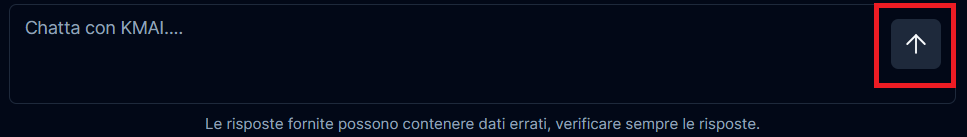
\includegraphics[width=0.8\textwidth]{buttoninserttextchat.png}
    \caption{Invio domanda}\label{fig:buttoninserttextchat}
\end{figure}
\subsubsection{Caricamento risposta chatbot}
Una volta inviata la domanda, il vostro messaggio vi apparirà nella parte dedicata alla chat, mentre sulla barra sottostante apparirà il simbolo di caricamento, che sta a indicare l'elaborazione in corso da parte del chatbot di un'eventuale risposta.
\begin{figure}[h!]
    \centering
    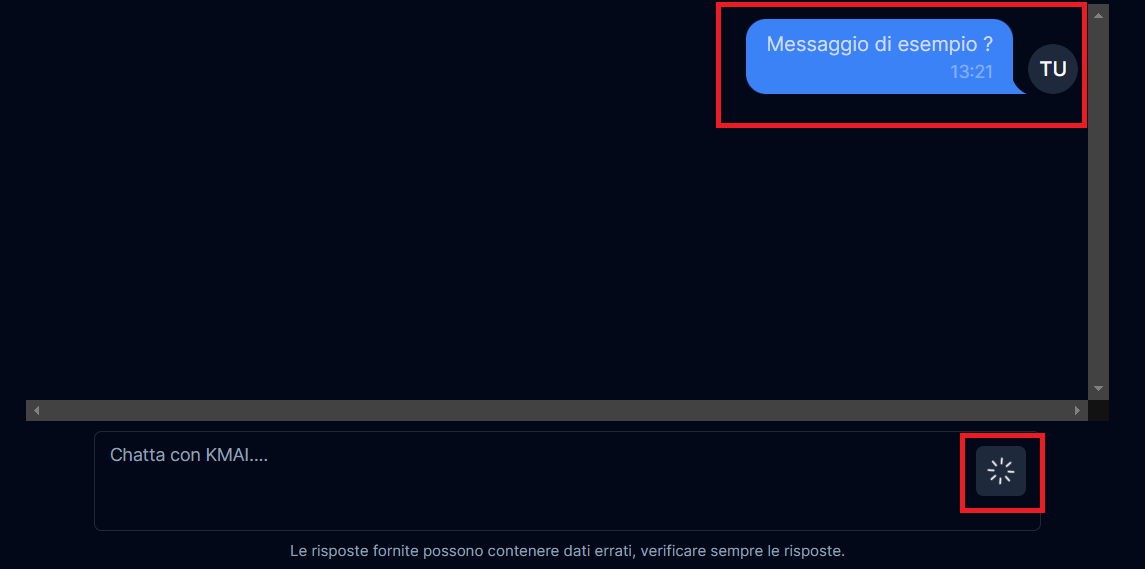
\includegraphics[width=0.8\textwidth]{loadingchatresponse.png}
    \caption{Caricamento risposta chatbot}\label{fig:loadingchatresponse}
\end{figure}
\subsubsection{Risposta chatbot}
Una volta completata la composizione della risposta il chatbot allegherà al messaggio di risposta le informazioni riguardante la fonte da cui ha raccolto i dati.\\
Qual ora fosse necessario, sarà possibile inoltre accedere direttamente alla fonte della risposta e quindi al file contenente le informazioni cliccando sul pulsante contenuto nel messaggio.
In caso si tratti di un pdf verrà aperto in un’altra cheda, altrimenti, se il file caricato è di un qualsiasi altro formato supportato dall’applicazione, verrà scaricato.
\begin{figure}[h!]
    \centering
    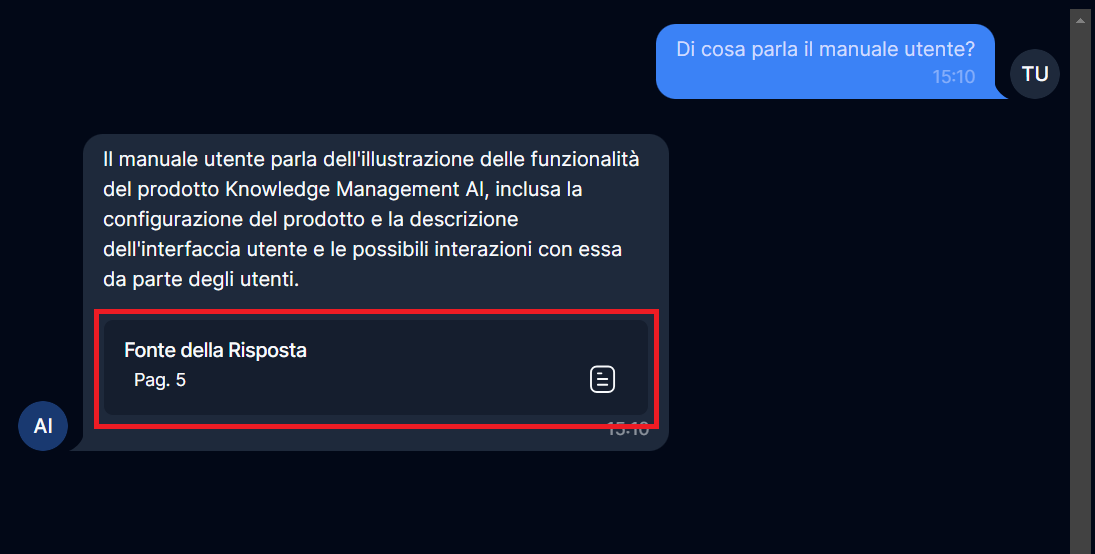
\includegraphics[width=0.8\textwidth]{rispostachat.png}
    \caption{Risposta chatbot}\label{fig:rispostachat}
\end{figure}

\newpage
\subsection{Gestione chat}
\subsubsection{Creazione automatica nuova chat}
Una volta inviato un primo messaggio al chatbot, quest'ultimo creerà in qutomatico una nuova chat impostando come titolo il testo del messaggio inviato.
\begin{figure}[h!]
    \centering
    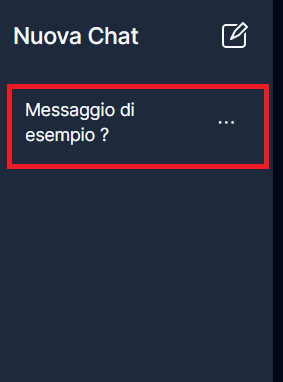
\includegraphics[width=0.3\textwidth]{automaticcreationchat.png}
    \caption{Creazione automatica nuova chat}\label{fig:automaticcreationchat}
\end{figure}

\subsubsection{Creazione nuova chat}
Qual'ora si volesse creare una nuova chat è possibile farlo dall'apposito pulsante affianco alla scritta "Nuova chat" .
\begin{figure}[h!]
    \centering
    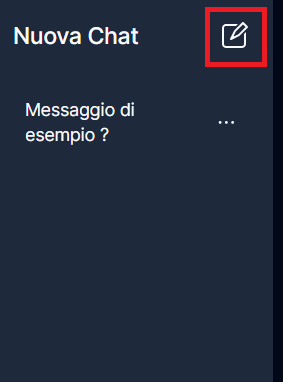
\includegraphics[width=0.3\textwidth]{createnewchat.png}
    \caption{Creazione nuova chat}\label{fig:createnewchat}
\end{figure}
\subsubsection{Eliminazione chat}
Qual'ora si volesse eliminare una chat archiviata è sufficiente premere sul pulsante a tre puntini affianco alla chat che si intende eliminare per poi premere il pulsante "Elimina".
\begin{figure}[h!]
    \centering
    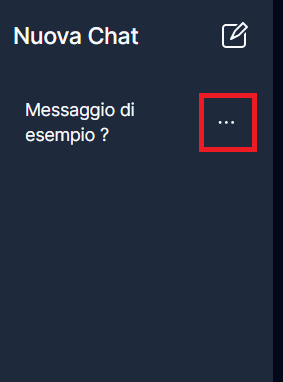
\includegraphics[width=0.3\textwidth]{deletechat.png}
    \caption{Eliminazione chat}\label{fig:deletechat}
\end{figure}
\\Per evitare eliminazioni accidentali, verrà richiesta una conferma prima di procedere.
\begin{figure}[h!]
    \centering
    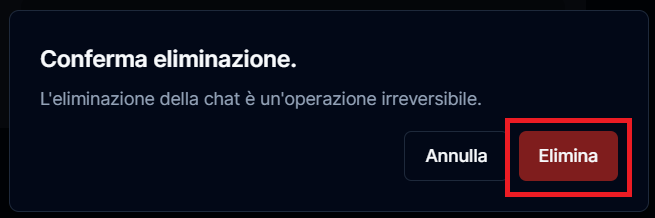
\includegraphics[width=0.6\textwidth]{confirmdeletechat.png}
    \caption{Conferma eliminazione chat}\label{fig:confirmdeletechat}
\end{figure}

\newpage
\subsection{Impostazioni applicazione}
Cliccando sulla rotellina presente nel menù di sinistra si apriranno le impostazioni dell'applicazione.
\begin{figure}[h!]
    \centering
    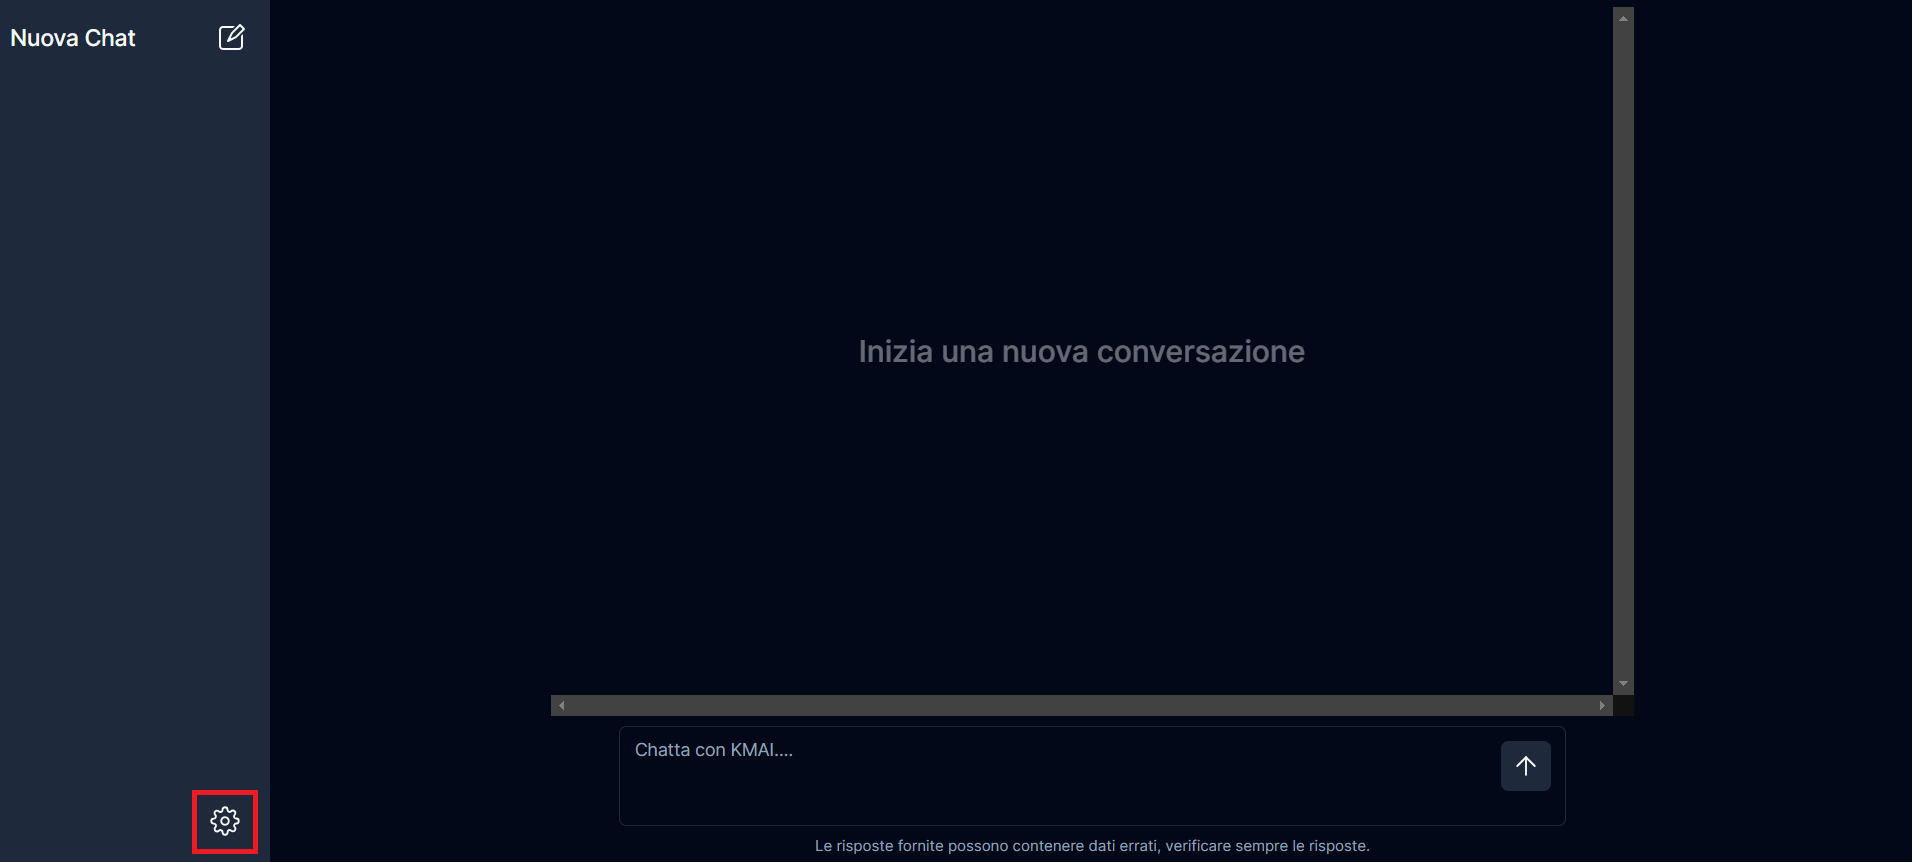
\includegraphics[width=0.8\textwidth]{schermatachatsetting.png}
    \caption{Impostazioni dell'applicazione}\label{fig:settingchat}
\end{figure}
\subsubsection{Modifica modello}
Dalle impostazioni è possibile scegliere il modello con cui fare domande sui documenti. Importante ricordare che i documenti caricati usando un modello locale non possono
essere interrogati con il chatbot che utilizza OpenAI e viceversa.
\begin{figure}[h!]
    \centering
    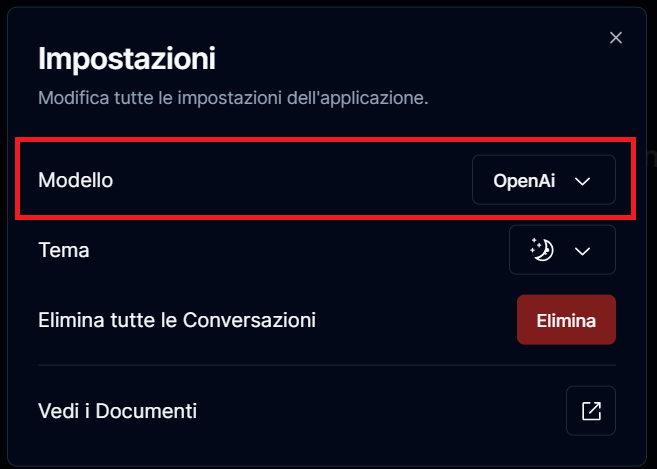
\includegraphics[width=0.364\textwidth]{settingchatmodel.png}
    \caption{Cambio modello}\label{fig:settingchatmodel}
\end{figure}

\newpage
\subsubsection{Elimina tutte le Conversazioni}
Cliccando nel pulsante "Elimina" è possibile eliminare tutte le conversazioni salvate fino a quel momento.
\begin{figure}[h!]
    \centering
    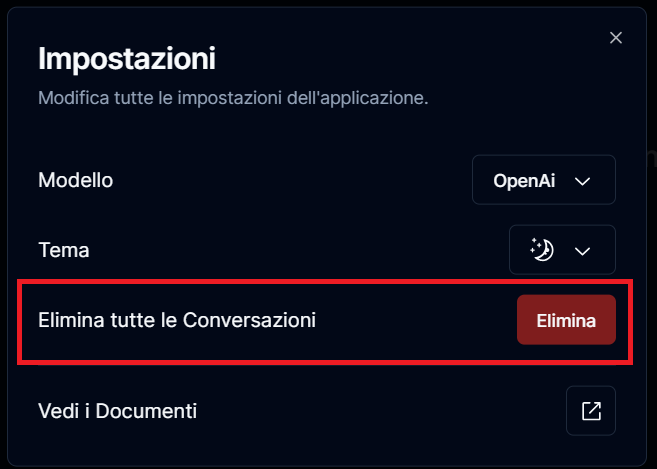
\includegraphics[width=0.364\textwidth]{deleteallchat.png}
    \caption{Elimina tutte le Conversazioni}\label{fig:deleteallchat}
\end{figure}
\\Per evitare eliminazioni accidentali, verrà richiesta una conferma prima di procedere.
\begin{figure}[h!]
    \centering
    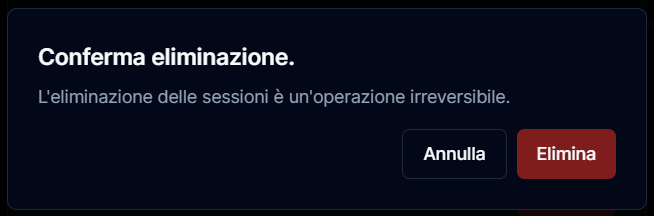
\includegraphics[width=0.6\textwidth]{confirmdeleteconversations.png}
    \caption{Conferma eliminazione Conversazioni}\label{fig:dialogdeleteconversation}
\end{figure}

\newpage
\subsubsection{Modifica tema}
È possibile cambiare il tema dell'applicazione selezionando tra modalità dark (rappresentata dalla luna) e modalità light (indicata dall'icona del sole).
\begin{figure}[h!]
    \centering
    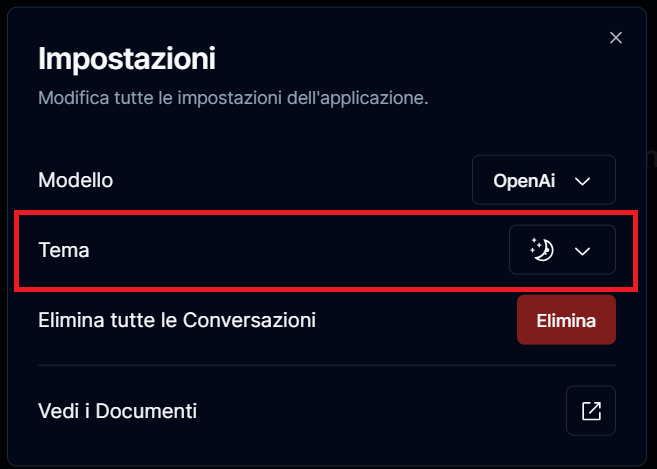
\includegraphics[width=0.364\textwidth]{settingchattheme.png}
    \caption{Cambio tema}\label{fig:settingchattheme}
\end{figure}
\subsubsection{Cambio pagina}
Per passare alla pagina documenti basta cliccare sul pulsante "Vedi i Documenti" presente in fondo alle impostazioni.
\begin{figure}[h!]
    \centering
    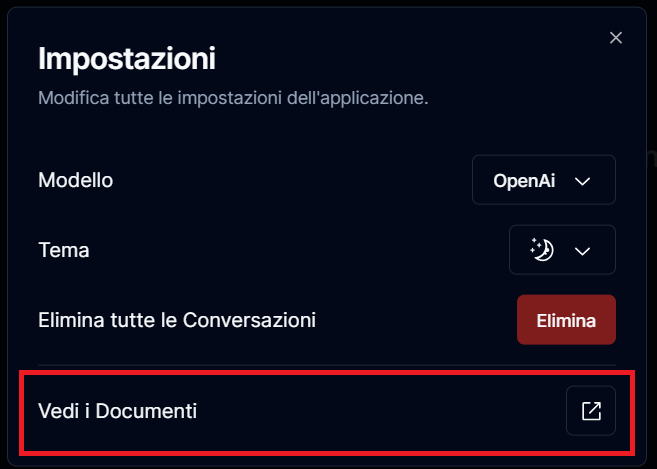
\includegraphics[width=0.364\textwidth]{settingchatchange.png}
    \caption{Vai alla pagina chat}\label{fig:changepage}
\end{figure}